\section{
    Корректность начально-краевой задачи для квазилинейной модели
}\label{sec:ch3:sec1}
%6_Chebotarev.pdf
%Mathematical modeling of complex heat transfer in
%the context of the endovenous laser ablation

\subsection{Введение}\label{subsec:ch3:sec1:subsec1}
Процедура эндовенозной лазерной абляции (EVLA) безопасна и достаточно эффективна при
лечении варикозного расширения вен.
Во время EVLA в поврежденную вену вводится лазерное оптическое волокно.
Затем лазерное излучение передается по волокну, которое в это время вытягивается из вены.
Конец оптического волокна обычно покрыт карбонизированным слоем (наконечник оптического волокна).
Карбонизированный слой разделяет лазерную энергию на нагрев кончика волокна и излучение.
Тепло от наконечника волокна передается через кровь и окружающие ткани за счет кондуктивной теплопередачи.
Теплообмен значительно увеличивается за счет потока пузырьков, образующихся на нагретом кончике волокна.
Излучение, попадающее в кровь и окружающие ткани, частично поглощается с выделением тепла.
В результате генерируемая тепловая энергия вызывает значительный нагрев вены, что приводит к ее облитерации.

Основными эффектами, которые обычно учитываются при моделировании ЭВЛА, являются кондуктивный перенос тепла,
перенос и поглощение излучения с выделением тепла, а также перенос тепла потоком пузырьков, образующихся
на конце горячего волокна.
В работах на основе оценки экспериментальных данных теплообмен потоком пузырьков моделируется
зависимостью коэффициента теплопроводности от температуры следующим образом: когда температура
в некоторой точке достигает и выше коэффициент теплопроводности увеличивается в 200 раз.
Такой подход при моделировании ЭВЛА применяется в [2], где доказана однозначная разрешимость
начально-краевой задачи для квазилинейной модели ЭВЛА, и в [12, 13], где исследуются экстремальные задачи ЭВЛА.

В настоящей работе мы изучаем обобщение модели EVLA, рассмотренной в [2].
В дополнение к вышеупомянутым эффектам мы также учитываем излучение абсолютно черного тела.
Это дает дополнительные нелинейные члены в уравнениях ЭВЛА. Доказана однозначная разрешимость
начально-краевой задачи и установлена сходимость итерационного алгоритма.
Работоспособность алгоритма иллюстрируется численными примерами.

\subsection{Formulation of the initial-boundary value problem}\label{subsec:ch3:sec1:subsec2}

Рассмотрим следующую начально-краевую задачу
в ограниченной трехмерной области $\Omega$ с
отражающей границей $\Gamma=\partial \Omega$:
\[
    \begin{gathered}
        \sigma \partial \theta / \partial t-\operatorname{div}(k(\theta) \nabla \theta)
        +b\left(\theta^{3}|\theta|-\varphi\right)=f \\
        -\operatorname{div}(\alpha \nabla \varphi)+
        \beta\left(\varphi-\theta^{3}|\theta|\right)=g, x \in \Omega, 0<t<T \\
        k(\theta) \partial_{n} \theta + p\left(\theta-\theta_{b}\right)|_{\Gamma}=0,
        \quad \alpha \partial_{n} \varphi
        + \gamma\left(\varphi-\theta_{b}^{4}\right)|_{\Gamma}=0,
        \quad \theta|_{t=0}=\theta_{i n}.
    \end{gathered}
\]


Здесь $\theta$ — нормированная температура, $\varphi$ — нормированная интенсивность излучения,
усредненная по всем направлениям.
Нормирующими множителями для получения из
$\theta$ и $\varphi$ абсолютной температуры и средней интенсивности излучения
являются $\mathcal{M}_{\theta}$ и $\mathcal{M}_{\varphi}$ соответственно.


Положительные параметры $b, \alpha, \beta, \gamma, p$ описывают радиационные
и теплофизические свойства среды [7], $\sigma(x, t)$ - произведение
удельной теплоемкости на объем плотность, $k(\theta)$ — коэффициент теплопроводности,
$f$ и $g$ описывают вклад источников тепла и излучения соответственно.
Символом $\partial_{n}$ обозначена производная по направлению внешней
нормали $\mathbf{n}$ к границе $\Gamma$.
Предположим,
что $\Omega$ — липшицева ограниченная область,
$\Gamma=\partial \Omega, Q=\Omega \times(0, T), \Sigma=\Gamma \times(0, T)$.


Обозначим через $L^{p}, 1 \leq p \leq \infty$ пространство Лебега, через $H^{1}$
пространство Соболева $W_{2}^{1}$ и через $L^ {p}(0, T ; X)$ пространство
Лебега функций из $L^{p}$, определенных на $(0, T)$, со значениями в банаховом пространстве $X$.
Пусть $H=L^{2}(\Omega), V=H^{1}(\Omega)$, а пространство $V^{\prime}$ двойственно к $V$.
Тогда мы отождествим $H$ с его двойственным пространством $H^{\prime}$ таким,
что $V \subset H=H^{\prime} \subset V^{\prime}$, и обозначим через $\|\cdot \|$ норму в $H$,
а через $(h, v)$ значение функционала $h \in V^{\prime}$ на элементе $v \in V$,
совпадающее со скалярным произведением в $ H$, если $h \in H$.


Будем далее предполагать, что исходные данные удовлетворяют следующим условиям:

(i) $\alpha, \beta, \sigma \in L^{\infty}(\Omega), b=r \beta, r=$ Const $>0;
\alpha \geq \alpha_{0}, \beta \geq \beta_{0},
\sigma \geq \sigma_{0}, \alpha_{0}, \beta_{0}, \sigma_{0}=$ Const $>0$.

(ii) $0<k_{0} \leq k(s) \leq k_{1},\left|k^{\prime}(s)\right| \leq k_{2}, s \in \mathbb{R},
\quad k_{j}=$ Const.

(iii) $0 \leq \theta_{b} \in L^{\infty}(\Sigma), 0 \leq \theta_{i n} \in L^{\infty}(\Omega);
\gamma_{0} \leq \gamma \in L^{\infty}(\Gamma),
p_{0} \leq p \in L^{\infty}(\Gamma), \gamma_{0}, p_{0}=$ Const $>0$.

(iv) $0 \leq f, g \in L^{\infty}(Q)$.

Пусть

\[
    W=\left\{y \in L^{2}(0, T ; V): \sigma y^{\prime}=\sigma d y / d t \in L^{2}\left(0, T, V^{\prime}\right)\right\}
\]

Определим операторы $A_{1}: V \rightarrow V_{0}^{\prime}$ и $A_{2}: V \rightarrow V^{\prime}$ такие,
что для всех $\theta, \varphi v$ справедливы следующие равенства:

\[
    \begin{gathered}
        \left(A_{1}(\theta), v\right)=(k(\theta) \nabla \theta, \nabla v)
        +\int_{\Gamma} p \theta v d \Gamma=(\nabla h(\theta), \nabla v)+\int_{\Gamma} p \theta v d \Gamma, \\
        \left(A_{2} \varphi, v\right)=(\alpha \nabla \varphi, \nabla v)
        +\int_{\Gamma} \gamma \varphi v d \Gamma,
    \end{gathered}
\]
где
\[
    h(s)=\int_{0}^{s} k(r) d r
\]

\textbf{Определение 1.}
Пара $\theta \in W, \varphi \in L^{2}(0, T ; V)$ называется слабым решением задачи (1) - (3), если

\[
    \begin{gathered}
        \sigma \theta^{\prime}+A_{1}(\theta)+b\left([\theta]^{4}-\varphi\right)=f_{b}+f
        \quad \text { a. e. on }(0, T), \quad \theta(0)=\theta_{i n}, \\
        A_{2} \varphi+\beta\left(\varphi-[\theta]^{4}\right)=g_{b}+g \quad \text { a. e. on }(0, T).
    \end{gathered}
\]

Здесь, $f_{b}, g_{b} \in L^{2}\left(0, T ; V^{\prime}\right)$ и

\[
    \left(f_{b}, v\right)=\int_{\Gamma} p \theta_{b} v d \Gamma,
    \quad\left(g_{b}, v\right)=\int_{\Gamma} \gamma \theta_{b}^{4} v d \Gamma \quad \forall v \in V
\]

\textit{Замечание 1.}
Так как $\theta \in W$, то $\theta \in C([0, T] ; V)$.
Следовательно, начальное условие имеет смысл.

\subsection{Iterative method}\label{subsec:ch3:sec1:subsec3}
Определим операторы
$F_{1}: L^{\infty}(\Omega) \rightarrow V$ и $F_{2}: L^{\infty}(Q) \times L^{2}(0, T ;V) \rightarrow W$
следующим образом.


Пусть $\varphi=F_{1}(\theta)$, если

\[
    A_{2} \varphi+\beta\left(\varphi-[\theta]^{4}\right)=g_{b}+g
\]
и $\theta=F_{2}(\zeta, \varphi)$ если

\[
    \sigma \theta^{\prime}+A(\zeta, \theta)+b\left([\theta]^{4}-\varphi\right)=f_{b}
    +f \quad \text { a. e. on }(0, T), \quad \theta(0)=\theta_{i n}.
\]


Здесь

\[
    (A(\zeta, \theta), v)=(k(\zeta) \nabla \theta, \nabla v)
    +\int_{\Gamma} p \theta v d \Gamma \quad \forall v \in V
\]


Пусть $w(t)=M_{0}+M_{1} t, t \in[0, T]$, где

\[
    \begin{gathered}
        M_{0}=\max \left\{\left\|\theta_{b}\right\|_{L^{\infty}(\Sigma)},
        \left\|\theta_{i n}\right\|_{L^{\infty}(\Omega)}\right\} \\
        M_{1}=\sigma_{0}^{-1}\left(\|f\|_{L^{\infty}(Q)}+\max b M_{2}\right),
        \quad M_{2}=\beta_{0}^{-1}\|g\|_{L^{\infty}(Q)} .
    \end{gathered}
\]



\textbf{Лемма 1.}
Пусть выполнены условия (i) - (iv), $0 \leq \theta \leq w(t), \varphi=F_{1}(\theta)$.
В таком случае
\[
    0 \leq \varphi \leq w^{4}(t)+M_{2}
\]


\textit{Доказательство.}
Умножая (6) в смысле внутреннего произведения $H$ на
$\psi=\max \left\{\varphi-M_{2}-w^{4}, 0\right\} \in$ $L^{2}(0, T ; V)$, получаем

\[
    \left(A_{2} \varphi-g_{b}, \psi\right)+\left(\beta\left(\varphi-M_{2}-[\theta]^{4}\right),
    \psi\right)=\left(g-\beta M_{2}, \psi\right) \leq 0.
\]


Заметим, что с учетом ограничений на $\theta$ выполняются следующие неравенства:

\[
    \begin{gathered}
        \left(A_{2} \varphi-g_{b}, \psi\right)=(\alpha \nabla \psi, \nabla \psi)+\int_{\Gamma} \gamma\left(\varphi-\theta_{b}^{4}\right) d \Gamma \geq(\alpha \nabla \psi, \nabla \psi) \\
        \left(\beta\left(\varphi-M_{2}-[\theta]^{4}\right), \psi\right)=(\beta \psi, \psi)+\left(\beta\left(w^{4}-[\theta]^{4}\right), \psi\right) \geq(\beta \psi, \psi) .
    \end{gathered}
\]


Таким образом, $\psi=0$ и $\varphi \leq w^{4}+M_{2}$.

Далее, умножая (6) в смысле скалярного произведения $H$ на $\xi=\min \{\varphi, 0\} \in$ $L^{2}(0, T ; V) $ аналогично получаем, что $\xi=0$. Таким образом, $\varphi\geq 0$.

\textbf{Лемма 2.}
Пусть выполняются условия (i)-(iv), $0 \leq \varphi \leq w^{4}(t)+M_{2}, \theta=F_{2}(\zeta, \varphi) , \zeta \in L^{\infty}(Q)$. Тогда $0 \leq \theta \leq w(t)$.

\textit{Доказательство.}
Пусть $\widehat{\theta}=\theta-w$. Перепишем уравнение (7) следующим образом
\[
    \sigma \widehat{\theta}^{\prime}+A(\zeta, \theta)
    -f_{b}+b\left([\widehat{\theta}+w]^{4}-
    \left(\varphi-M_{2}\right)\right)=f-\sigma M_{1}+b M_{2} \leq 0.
\]

Умножая (9) в смысле скалярного произведения $H$ на $\eta=\max \{\widehat{\theta}, 0\} \in W$.
Заметим, что значение правой части неположительно, а также

\[
    \begin{gathered}
        \left(\sigma \widehat{\theta}^{\prime}, \eta\right)=\left(\sigma \eta^{\prime}, \eta\right)=\frac{d}{2 d t}(\sigma \eta, \eta) \\
        \left(A(\zeta, \theta)-f_{b}, \eta\right)=(k(\zeta) \nabla \eta, \nabla \eta)+\int_{\Gamma} p\left(\widehat{\theta}+w-\theta_{b}\right) \eta d \Gamma \geq 0 \\
        \left([\widehat{\theta}+w]^{4}-w^{4}\right) \max \{\widehat{\theta}, 0\} \geq 0, \quad\left(w^{4}+M_{2}-\varphi\right) \eta \geq 0
    \end{gathered}
\]


Тогда

\[
    \frac{d}{d t}(\sigma \eta, \eta) \leq 0,\left.\quad \eta\right|_{t=0}=0
\]

Таким образом, $\eta=0, \widehat{\theta} \leq 0, \theta \leq w$. Аналогично, умножая (9) в смысле скалярного произведения $H$ на $\eta=\min \{\theta, 0\} \in W$, получаем, что $\eta=0, \quad \theta \geq 0$.

Пусть $\theta_{0}=\theta_{i n}, \quad \varphi_{0}=F_{1}\left(\theta_{0}\right)$.
Определим рекурсивно последовательности $\theta_{m} \in W, \varphi_{m} \in L^{2}(0, T ; V)$ таким образом, что

\[
    \theta_{m}=F_{2}\left(\theta_{m-1}, \varphi_{m-1}\right),
    \quad \varphi_{m}=F_{1}\left(\theta_{m}\right), \quad m=1,2, \ldots
\]


Из лемм 1 и 2 следуют оценки

\[
    0 \leq \varphi_{m} \leq w^{4}(t)+M_{2}, \quad 0 \leq \theta_{m} \leq w(t), \quad m=1,2, \ldots
\]

\textbf{Лемма 3.} Пусть выполнены условия (i) — (iv). Тогда существует константа $C>0$, не зависящая от $m$, такая, что

\[
    \begin{gathered}
        \left\|\varphi_{m}\right\|_{L^{2}(0, T ; V)} \leq C, \quad\left\|\theta_{m}\right\|_{L^{2}(0, T ; V)} \leq C, \\
        \int_{0}^{T-\delta}\left\|\theta_{m}(s+\delta)-\theta_{m}(s)\right\|^{2} d s \leq C \delta .
    \end{gathered}
\]


\textit{Доказательство.}
Из определения последовательностей $\varphi_{m}, \theta_{m}$ следуют равенства

\[
    \begin{gathered}
        A_{2} \varphi_{m}+\beta\left(\varphi_{m}-\left[\theta_{m}\right]^{4}\right)=g_{b}+g \\
        \sigma \theta_{m}^{\prime}+A\left(\theta_{m-1},
        \theta_{m}\right)+b\left(\left[\theta_{m}\right]^{4}-\varphi_{m-1}\right)=f_{b}+f
        \quad \text { a. e. on }(0, T), \quad \theta_{m}(0)=\theta_{i n}.
    \end{gathered}
\]


Оценки (12) выводятся стандартным образом из уравнений (14) и (15) и с учетом (11),
т.е. ограниченности последовательностей в $L^{\infty}(Q)$.

Получим оценку, гарантирующую компактность последовательности $\theta_{m}$ в $L^{2}(Q)$.
Перепишем (15) как

\[
    \sigma \theta_{m}^{\prime}=\chi_{m} \text { a.e. on }(0, T), \quad \theta_{m}(0)=\theta_{i n}
\]


где

\[
    -\chi_{m}=A\left(\theta_{m-1},
    \theta_{m}\right)+b\left(\left[\theta_{m}\right]^{4}
    -\varphi_{m-1}\right)-f_{b}-f.
\]
Отметим, что с учетом полученных оценок последовательность
$\chi_{m}$ ограничена в $L^{2}\left(0, T ; V^{\prime}\right)$.
Умножим (16) в смысле скалярного произведения произведения $H$ на $\theta_{m}(t)-\theta_{m}(s)$
и проинтегрируем по $t$ на интервале $(s, s+\delta)$ и
над $s$ на $(0, T-\delta)$, предполагая, что $\delta>0$ достаточно мало.
В результате получим
\[
    \frac{1}{2} \int_{0}^{T-\delta}\left\|\sqrt{\sigma}\left(\theta_{m}(s+\delta)
    - \theta_{m}(s)\right)\right\|^{2} d s
    = \int_{0}^{T-\delta} \int_{s}^{s+\delta} c_{m}(t, s) d t d s
\]


где

\[
    c_{m}(t, s)=\left(\chi_{m}(t), \theta_{m}(t)-\theta_{m}(s)\right)
    \leq\left\|\chi_{m}(t)\right\|_{V^{\prime}}^{2}
    +\frac{1}{2}\left\|\theta_{m}(t)\right\|_{V}^{2}
    +\frac{1}{2}\left\|\theta_{m}(s)\right\|_{V}^{2}.
\]

Для оценки интегралов от слагаемых, зависящих от $t$, достаточно изменить порядок интегрирования.
Используя ограниченность последовательностей
$\theta_{m}$ в $L^{2}(0, T ; V)$ и $\chi_{m}$ в $L^{2}\left(0, T ; V^{\prime}\right)$,
получаем оценку равностепенной непрерывности (13).

Полученные оценки (12), (13) позволяют утверждать, переходя при необходимости к подпоследовательностям,
что существуют функции $\theta_{*}, \varphi_{*}$ такие, что

\[
    \begin{aligned}
        \theta_{m} \rightarrow \widehat{\theta} \text { weakly in } L^{2}(0, T ; V), \text { strongly in } L^{2}(0, T ; H), \\
        \varphi_{m} \rightarrow \widehat{\varphi} \text { weakly in } L^{2}(0, T ; V) .
    \end{aligned}
\]

Сходимости (17) достаточно, для перехода к пределу при $m \rightarrow \infty$
в равенствах (14), (15) и доказательства,
что предельные функции $\widehat{\theta}, \widehat{\varphi } \in L^{2}(0, T ; V)$ таковы,
что $\sigma \widehat{\theta}^{\prime} \in L^{2}\left(0, T ; V^{ \prime}\right)$
и для них выполняются равенства (4), (5).


\textbf{Теорема 1.}
Пусть выполнены условия (i)-(iv).
Тогда задача (1)-(3) имеет хотя бы одно решение.

\subsection{Uniqueness theorem and convergence of the iterative method}\label{subsec:ch3:sec1:subsec4}
Покажем, что в классе функций с ограниченным градиентом температуры решение единственно.
Это позволяет доказать сходимость итерационной процедуры.

\textbf{Теорема 2.}
Пусть выполнены условия (i)–(iv).
Если $\theta_{*}, \varphi_{*}$ — решение задачи (1)-(3) такое,
что $\theta_{*}, \nabla \theta_{*} \in L^{\infty }(Q)$, то других ограниченных решений этой задачи нет.

\textit{Доказательство.}

Пусть $\theta_{1}, \varphi_{1}$ - другое решение задачи (1) - (3),
$\theta=\theta_{1}-\theta_{*}, \varphi=\varphi_{ 1}-\varphi_{*}$.
В таком случае

\[
    \begin{gathered}
        \sigma \theta^{\prime}+A_{1}\left(\theta_{1}\right)
        -A_{1}\left(\theta_{*}\right)+b\left(\left[\theta_{1}\right]^{4}-
        \left[\theta_{*}\right]^{4}-\varphi\right)=0 \quad \text { a. e. on }(0, T), \quad \theta(0)=0 . \\
        A_{2} \varphi+\beta\left(\varphi-\left(\left[\theta_{1}\right]^{4}
        -\left[\theta_{*}\right]^{4}\right)\right)=0 \quad \text { a. e. on }(0, T).
    \end{gathered}
\]



Умножьте (18) в смысле внутреннего произведения $H$ на $\theta$ и проинтегрируйте по времени.
Как результат
\[
    \frac{1}{2}\|\sqrt{\sigma} \theta\|^{2}+
    \int_{0}^{t}\left(\left(k\left(\theta_{1}\right) \nabla \theta,
    \nabla \theta\right)+\int_{\Gamma} p \theta^{2}(s) d \Gamma\right) d s=
\]
\[
    -\int_{0}^{t}\left(b\left(\left[\theta_{1}\right]^{4}-\left[\theta_{*}\right]^{4}-\varphi\right),
    \theta\right) d s-\int_{0}^{t}\left(\left(k\left(\theta_{1}\right)-k\left(\theta_{*}\right)\right)
    \nabla \theta_{*}, \nabla \theta\right) d s
\]

Пусть $\left|\theta_{1}\right| \leq M,\left|\theta_{*}\right| \leq M$.
С учетом ограничения на функцию $k$ получаем неравенство

\[
    \begin{aligned}
        \frac{\sigma_{0}}{2}\|\theta\|^{2}+k_{0} & \int_{0}^{t}\|\nabla \theta\|^{2} d s \leq \\
        & \int_{0}^{t}\left(4 M \max b\|\theta\|^{2}+\|\varphi\|\|\theta\|\right) d s
        +k_{2}\left\|\nabla \theta_{*}\right\|_{L^{\infty}(Q)} \int_{0}^{t}\|\theta\|\|\nabla \theta\| d s.
    \end{aligned}
\]


Принимая во внимание, что
$\|\theta\|\|\nabla \theta\| \leq \varepsilon\|\nabla \theta\|^{2}+
\frac{1}{4 \varepsilon}\|\theta\|^{2}$
и предполагая
\[
    \varepsilon=\frac{k_{0}}{k_{2}\left\|\nabla \theta_{*}\right\|_{L^{\infty}(Q)}}
\]


из (20) получаем

\[
    \frac{\sigma_{0}}{2}\|\theta\|^{2} \leq \int_{0}^{t}
    \left(4 M \max b\|\theta\|^{2}+\|\varphi\|\|\theta\|\right) d s
    +\frac{1}{4 \varepsilon} k_{2}\left\|\nabla \theta_{*}\right\|_{L^{\infty}(Q)}
    \int_{0}^{t}\|\theta\|^{2} d s.
\]


Умножьте (19) на $\varphi$ в смысле скалярного произведения $H$.
Как результат

\[
    \left(A_{2} \varphi, \varphi\right)+(\beta \varphi, \varphi)=
    \left(\beta\left(\left[\theta_{1}\right]^{4}-\left[\theta_{2}\right]^{4}\right), \varphi\right)
    \leq 4 \max \beta M^{3}\|\theta\|\|\varphi\|.
\]


Следовательно, $\|\varphi\| \leq 4 \beta_{0}^{-1} \max \beta M^{3}\|\theta\|$.
Тогда из (21) и неравенства Гронуолла следует, что $\theta=0, \theta_{1}$
совпадает с $\theta_{*}$ и, соответственно, $\varphi_{1}$ совпадает с $\varphi_{*}$.

\textbf{Теорема 3.}

Пусть выполнены условия (i)-(iv).
Если $\theta_{*}, \varphi_{*}$ — решение задачи (1)-(3) такое,
что $\theta_{*}, \nabla \theta_{*} \in L^{\infty }(Q)$,
то для последовательностей (10) имеют место следующие сходимости:

\[
    \theta_{m} \rightarrow \theta_{*} \text { in } L^{2}(0, T ; V),
    \quad \varphi_{m} \rightarrow \varphi_{*} \text { in } L^{2}(0, T ; V).
\]


\textit{Доказательство.}

Сначала покажем, что $\theta_{m} \rightarrow \theta_{*}$ в $L^{2}(0, T ; H)$.
Предполагая противное, заключаем, что существуют $\varepsilon_{0}>0$ и подпоследовательность
$\theta_{m^{\prime}}$ такие, что
$\left\|\theta_{m^{\prime}} -\theta_{*}\right\|_{L^{2}(0, T ; H)} \geq \varepsilon_{0}$.
Оценки (12), (13) позволяют утверждать, переходя при необходимости к подпоследовательностям,
что справедливы результаты сходимости (17), где $\widehat{\theta}, \widehat{\varphi}$
также является решением задачи (1) - (3).
Следовательно, $\left\|\widehat{\theta}-\theta_{*}\right\|_{L^{2}(0, T ; H)} \geq \varepsilon_{0}$,
что противоречит теореме 2 о единственности решения.
Из уравнений (14) и (15) с учетом (11), т.е. ограниченности последовательностей в $L^{\infty}(Q)$,
а также доказанной сходимости $\theta_{m}$ в $L^{2}(0, T ; H)$
следует сходимость $\theta_{m} \rightarrow \theta_{*}, \varphi_{m} \rightarrow \varphi_{*}$ в $L^ {2}(0, Т; V).$

\subsection{Numerical simulation}\label{subsec:ch3:sec1:subsec5}

Перенос тепла и излучения будем рассматривать в среде, состоящей из четырех частей,
которые интерпретируются как кровь, стенки вены, предвенозная ткань и оптическое волокно.
Расчетная область в цилиндрической системе координат в случае угловой симметрии схематизирована
на рис. 1 (линейные размеры даны в миллиметрах).

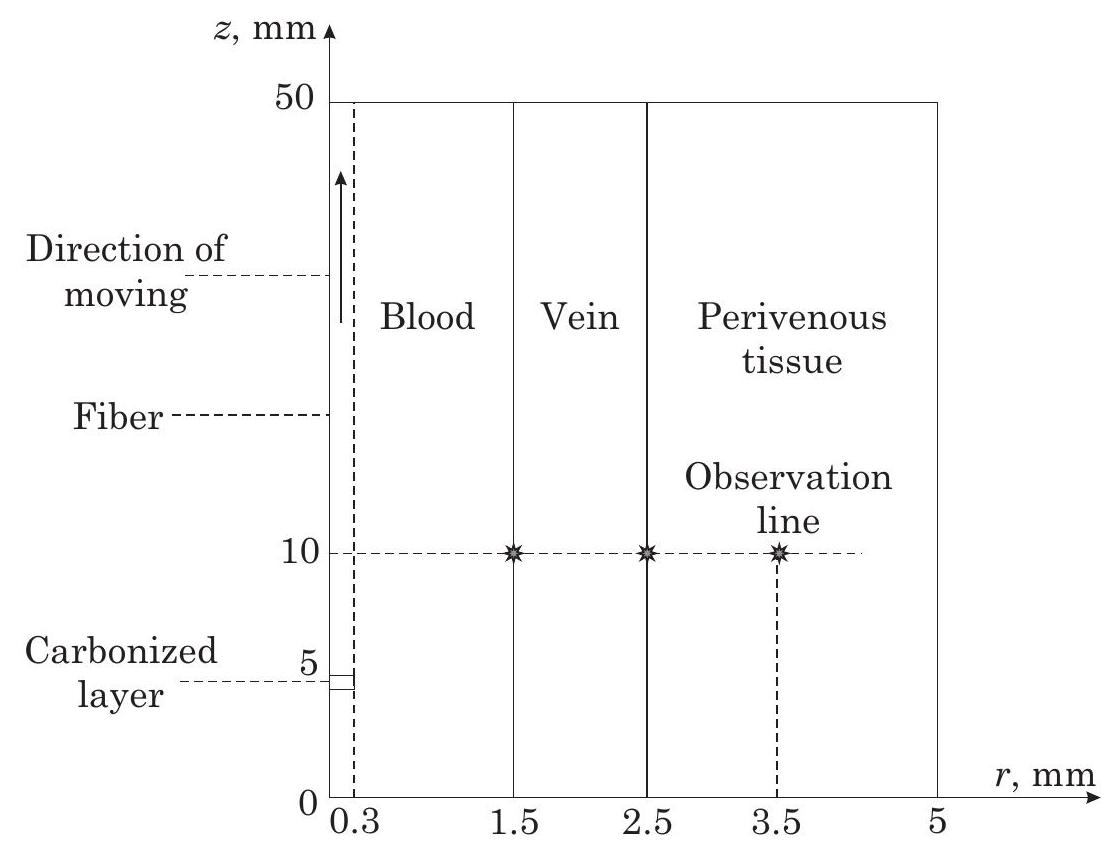
\includegraphics[height=3.5cm]{images/6_chebotarev.jpg}
Рисунок 1: Вычислительная область.

Для нахождения решения начально-краевой задачи (1) - (3) дискретизируем
интервал времени $(0, T), \quad 0=t_{0}<t_{1}<t_{2}< \ldots<t_{N}=T$.
Для каждого момента времени $t=t_{l}=l \Delta t$, $l=1,2, \ldots, N$
используется итерационный алгоритм для нахождения решения соответствующей краевой задачи.
$n$-й шаг итерационной процедуры $(n=1,2,\ldots,M)$ записывается следующим образом

\[
    \begin{gathered}
        -\operatorname{div}\left(\alpha \nabla \varphi_{n}\right)
        +\beta\left(\varphi_{n}-\theta_{n-1}^{3}\left|\theta_{n-1}\right|\right)=g, \\
        \sigma \partial \theta_{n} / \partial t
        -\operatorname{div}\left(k\left(\theta_{n-1}\right) \nabla \theta_{n}\right)
        -b\left(\theta_{n-1}^{3}\left|\theta_{n}\right|-\varphi_{n}\right)=f, \quad x \in \Omega, \\
        k\left(\theta_{n-1}\right) \partial_{n} \theta_{n}+
        \left.p\left(\theta_{n}-\theta_{b}\right)\right|_{\Gamma}=0,
        \quad \alpha \partial_{n} \varphi_{n}+\left.\gamma\left(\varphi_{n}-\theta_{b}^{4}\right)\right|_{\Gamma}=0,
    \end{gathered}
\]


где производная по времени в (23) аппроксимируется следующим образом

\[
    \frac{\partial \theta_{n}}{\partial t} \simeq \frac{\left.\theta_{n}\right|_{t=t_{l}}
        -\left.\theta_{M}\right|_{t=t_{l-1}}}{\Delta t}
\]

а функции $\theta_{n}, \theta_{n-1}, \varphi_{n}$ в (22) - (24) являются приближениями решения,
соответствующего моменту времени $t=t_{l}$.
Нижний индекс функций $\theta_{n}, \theta_{n-1}$ и $\varphi_{n}$ означает номер итерации.
Для инициализации итерационной процедуры задаем начальное приближение температуры для каждого момента времени:

\[
    \left.\theta_{0}\right|_{t=t_{l}}=\left.\theta_{M}\right|_{t=t_{l-1}},
    \quad l=1,2, \ldots, N,\left.\quad \theta_{M}\right|_{t=t_{0}}=\theta_{i n}.
\]


В уравнениях (22) и (23)
$g=P_{\varphi} \chi / \mathcal{M}_{\varphi}, f=P_{\theta} \chi / \mathcal{M}_{ \theta},$
где $P_{\varphi}$ — мощность источника, затрачиваемая на излучение, $P_{\theta}$ описывает мощность источника,
затрачиваемая на нагрев кончика световода, $\chi$ — характеристика функция части среды,
в которой находится кончик волокна, деленная на объем конца волокна,
$\mathcal{M}_{\varphi}$ и $\mathcal{M}_{\theta}$ являются нормирующими коэффициенты для получения
из $\varphi$ и $\theta$ средней интенсивности излучения и абсолютной температуры.

Для реализации каждого шага итерационного алгоритма (22)-(25) использовался метод конечных
элементов с использованием пакета программ FreeFEM++ [14].
Оптические и теплофизические параметры среды взяты из [10].
Параметры $\theta_{b}$ и $\theta_{i n}$ соответствуют температуре $37^{\circ}\mathrm{C}$,
а коэффициент $\gamma$ равен 1.
Во всех расчетах начальное положение кончика оптического волокна соответствует
$(r, z)=(0,5)$, а скорость его обратного хода равна $2 \mathrm{~mm} / \mathrm{s}$.
Следуя [10, 11], моделируем перенос тепла потоком пузырьков, образующихся на конце горячего волокна,
через коэффициент теплопроводности в зависимости от температуры следующим образом:
при достижении температуры в некоторой точке $95^{\circ} \ mathrm{C}$ и выше коэффициент
теплопроводности увеличивается в 200 раз.

Эффективность лазерной абляции можно оценить по поведению профилей
температуры в различных точках расчетной области.
Основными параметрами процедуры лазерной абляции являются мощность лазера, длина волны излучения,
скорость обратного хода оптического волокна и соотношение мощностей лазера,
затрачиваемых на излучение и нагрев кончика волокна.
Отметим, что решение задачи (1) - (3) зависит от длины волны неявно,
параметрами $\alpha$ и $\beta$, описывающими радиационные свойства среды
(см~. таблицы значений коэффициента поглощения и приведенный коэффициент рассеяния,
определяющий параметры $\alpha$ и $\beta[10,11])$.
Как правило, лазерная абляция осуществляется излучением с длиной волны от 810 до $1950 \mathrm{~нм}$.
Достаточно широко используемые диапазоны скорости отвода волокна и
мощности лазерного излучения составляют
$1-3 \mathrm{~mm}/\mathrm{s}$ и $5-15 \mathrm{~W}$ соответственно $[9, 10,11]$.

На рис~. 2 показано поведение профилей температуры в точке $(1.5,10)$
для излучения с разными длинами волн: $810 \mathrm{~нм}, 1064 \mathrm{~нм}, 1470 \mathrm{~нм}$
и $1950 \mathrm{~nm}$.
Мощность источника задается как
$\left(P_{\varphi}, P_{\theta}\right)=(7 \mathrm{~W}, 3 \mathrm{~W})$ во всех случаях.
Как видно из рис. 2, существенное влияние на поведение температурного профиля
оказывает изменение длины волны излучения.
Тем не менее можно обеспечить достаточно близкую продолжительность кипения
(при температуре более $95^{\circ}\mathrm{C}$)
для температурных профилей, соответствующих разным длинам волн, путем изменения
мощности лазера $P=P_{\ varphi}+P_{\theta}$,
сохраняя отношение $P_{\varphi}/P_{\theta}$ равным $7/3$ (см. рис. 3).

Отметим, что расчетная температура в точках околовенозной ткани
$(2,5,10)$ и $(3,5,10)$ вполне безопасна (см. рис. 4).

Как видно из проведенных экспериментов, использование компьютерного моделирования
является перспективным способом определения оптимальных параметров излучения,
обеспечивающих эффективное и безопасное проведение ЭВЛА.

